\documentclass[refman]{scrartcl}
% ----------------------------------------------------------------------------------------------------------
% HEADER
% ----------------------------------------------------------------------------------------------------------

\usepackage[english]{babel}
\usepackage[utf8]{inputenc}

\usepackage{fancyhdr}
\usepackage{graphicx}
\usepackage[dvipsnames]{xcolor} 
\usepackage{epigraph}

\usepackage{amsmath}
\usepackage{amsthm}
\usepackage{amssymb}

\usepackage{listings}

\pagestyle{fancy}

\theoremstyle{definition}
\newtheorem{definition}{Definition}
\newtheorem{lemma}{Lemma}
\newtheorem{exmp}{Example}
\newtheorem{remark}{Remark}
\newtheorem{theorem}{Theorem}

\begin{document}
%
% ----------------------------------------------------------------------------------------------------------
% TITLEPAGE & TABLE OF CONTENTS
% ----------------------------------------------------------------------------------------------------------
%
\begin{titlepage}
	\centering
	
\includegraphics[width=0.15\textwidth]{images/huberlin_logo}\par\vspace{1cm}
	{\scshape\LARGE Humboldt University of Berlin \par}
	\vspace{1cm}
	{\scshape\Large Einf{\"u}hrung in das wissenschaftliche Rechnen \par}
	\vspace{1.5cm}
	{\huge\bfseries Analysis of selected sorting Algorithms\par}
	\vspace{2cm}
	{\Large\itshape Christian Parpart \& Kei Thoma \par}
	\vfill

	\vfill

% Bottom of the page
	{\large \today\par}
\end{titlepage}

\tableofcontents
\newpage
%
% ----------------------------------------------------------------------------------------------------------
% CONTENTS
% ----------------------------------------------------------------------------------------------------------
%
% change section names later
\section{Introduction}
%
It is perhaps the most profound realization
\newpage
%
\section{Theoretical Results}
%
\subsection{Fundamental Definitions and Lemmas}
\begin{definition}
    Let \(z\) be an integer in the decimal system. To convert \(z\) to the \textit{binary system}, we have
    \begin{equation*}
        z := d_{n-2}d_{n-3}\dots d_1 d_2 = \sum_{i = 0}^{n-2}d_i 2^i
    \end{equation*}
    where \(d_i \in \{0, 1\}\) are digits. \cite{bib:rabus}
\end{definition}
%
\begin{lemma} \label{theo:bina}
    Let \(\beta \in \mathbb{N}, \beta \geq 2\) and \(x \in \mathbb{R}\) with \(x \neq 0\). Then there is one and only one representation for \(x\) in the form of
    \begin{equation*}
        x = (-1)^{\nu} \beta^N \sum_{i = 1}^{\infty}x_i \beta^{-i}
    \end{equation*}
    where \(\nu \in \{0, 1\}\); \(N \in \mathbb{Z}\); \(x_1 = 1\) and \(x_i \in \{0, 1, \dots , \beta - 1\}\); and for every \(n \in \mathbb{N}\) exists an index \(i \geq n\) with \(x_i \neq \beta - 1\). \cite{bib:rabus}
\end{lemma}
%
\begin{definition}
    \(x\) is a normalized t-digit long floating point number infty
    \begin{equation*}
        x = (-1)^{\nu} 2^N \sum_{i = 1}^{t}x_i 2^{-i} = (-1)^{\nu} 2^N \cdot (0.x_1 x_2 \dots x_t)_2
    \end{equation*}
    with \(\nu \in {0, 1}\); \(N_{\text{min}} \leq N \leq N_{\text{max}}\); \(N \in \mathbb{Z}\); \(x_i \in \{0, 1\}\) for all \(i = 2, \dots, t\) and \(x_1 = 1\).

    The number \(m = \sum_{i = 1}^{t}x_i 2^{-i} = (0.x_1 x_2 \dots x_t)_2\) is called mantissa of \(x\) and \(t\) is the mantissa length.  \cite{bib:rabus}
\end{definition}
We will see practical examples to convert decimal numbers to binary and back in section \ref{exmp:z1}.
\begin{remark}
There are special values reserved on the computer. These are \(+\infty\), \(-\infty\) and NaN (not a number).  \cite{bib:rabus}
\end{remark}
%
\begin{definition} \label{theo:round}
    Let \(t\) be the mantissa length. We define the rounding of \(x\) to a floating point as follows. \\
    If \(N_{\text{min}} \leq N \leq N_{\text{max}}\), then
    \begin{equation*}
        \text{rd}_t(x) :=
        \begin{cases}
            (-1)^{\nu} 2^N \sum_{i = 1}^{t}x_i 2^{-i} \text{ for } x_{t+1} = 0 \\
            (-1)^{\nu} 2^N (\sum_{i = 1}^{t}x_i 2^{-i} + 2^{-t}) \text{ for } x_{t+1} = 1 \\
        \end{cases}
    \end{equation*}
    If \(N \leq N_{\text{min}} - t\), then \(\text{rd}_t(x) := 0\). \\
    If \(N_{\text{min}} - t < N \leq N_{\text{min}}\), then
    \begin{equation*}
        \text{rd}_t(x) :=
        \begin{cases}
            (-1)^{\nu} 2^{N_{\text{min}}} \sum_{j = n + 1}^{t}x_{j-n} 2^{-j} \text{ for } x_{t+1-n} = 0 \\
            (-1)^{\nu} 2^{N_{\text{min}}} (\sum_{j = n + 1}^{t}x_{j-n} 2^{-i} + 2^{-t}) \text{ for } x_{t+1-n} = 1 \\
        \end{cases}
    \end{equation*}
    If \(|x| > x_{\text{min}}\), then we get an overflow and in most cases we continue with \(\infty\).  \cite{bib:rabus}
\end{definition}
%
\begin{lemma} \label{theo:margin}
    For absolute and relative error between a real number and its floating point representation we have the margin  \cite{bib:rabus}
    \begin{align*}
        e_{\text{abs}} &= | \text{rd}_t(x) - x | \leq 2^{N - t - 1} \\
        e_{\text{rel}} &= \left| \frac{\text{rd}_t(x) - x}{\text{rd}_t(x)} \right| \leq 2^{-t}
    \end{align*}
\end{lemma}
%
\begin{definition}
    \begin{equation*}
        \tau := \text{max} \left\{ \left| \frac{\text{rd}_t(x) - x}{x}\right|, \left| \frac{\text{rd}_t(x) - x}{\text{rd}_t(x)} \right| \right\} \leq 2^{-t} \\
    \end{equation*}
    is called the relative machine precision.  \cite{bib:rabus}
\end{definition}

\begin{theorem}
    The relative machine precision can be computed with the algorithm illustrated in figure \ref{fig:epsilon}.
    \begin{figure}[h]
        \centering
            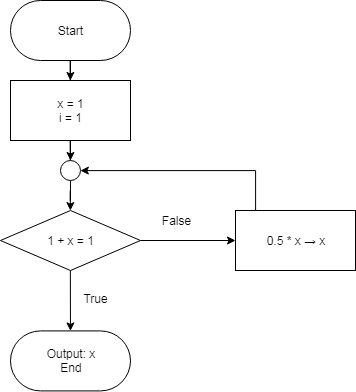
\includegraphics[width=0.4\textwidth]{graphics/machine_epsilon_flowchart}
        \caption{algorithm to find the relative machine precision}\label{fig:epsilon}
      \end{figure}
\end{theorem}

\begin{theorem}
    Using a computer, the relative machine precision can be computed in the following manner
    \begin{equation*}
        \tau = \left|\frac{7}{3} - \frac{3}{4} - 1\right|
    \end{equation*}
\begin{proof}
    We will first evaluate \(\frac{7}{3} - \frac{4}{3}\). We have
    \begin{align}
        \text{rd}_t(\frac{7}{3}) &= \text{rd}_t((10.\overline{01})_2) = \text{rd}_t((0.10\overline{01})_2 \times 2^2) \\
        \text{rd}_t(\frac{4}{3}) &= \text{rd}_t((1.\overline{01})_2) = \text{rd}_t((0.1\overline{01})_2 \times 2^1)
    \end{align}
    The decimal places of the two numbers only differ in placing. Therefore, if we wound the two numbers above one will be rounded up and the other will be rounded down, and we have
    \begin{equation*}
        \left|\text{rd}_t(\frac{7}{3}) - \text{rd}_t(\frac{4}{3})\right| = 2^2 \cdot \sum_{i=1}^{t} \frac{1}{2} - \frac{1}{4} + 0 + \dots + 0 + \frac{1}{2^t} = 1 + \frac{1}{2^t}
    \end{equation*}
    If we subtract \(1\) from the last term, we get \(\tau = \frac{1}{2^t}\) as desired.
\end{proof}
\end{theorem}
For all following examples, let the mantissa length be \(t = 8\) and the exponent of the floating point arithmetic be bounded by \(N_{\text{min}} = -5\) and \(N_{\text{max}} = 8\).
%
% ===================================================================
% (a)
% ===================================================================
%
\begin{exmp} \label{exmp:xmax}
    Given the context as defined above, the largest number that can be represented is \(x_\text{max} = 255\). The calculation is fairly simple; choose the largest exponent possible and fill every digit of the mantissa with ones. In binary, this would be
    \begin{equation*}
        x_\text{max} = (0.11111111)_2 \times 2^8 = (11111111)_2 \text{,}
    \end{equation*}
    or in decimal
    \begin{align*}
        x_\text{max} &= (-1)^{\nu} \cdot 2^N \cdot \sum_{i=1}^{t}x_i \beta^{-i}\\
        &= 2^8 \cdot \left(\frac{1}{2} + \frac{1}{4} + \frac{1}{8} + \frac{1}{16} + \frac{1}{32} + \frac{1}{64} + \frac{1}{128} + \frac{1}{256}\right) \\
        &= 255 \text{.}
    \end{align*}
\end{exmp}
\begin{exmp}
    To find the smallest possible normalized positive value in the defined floating point arithmetic, we proceed similary to the example \ref{exmp:xmax}. Set the exponent as small as possible and fill the mantissa with zero but the first place. We have in binary
    \begin{equation*}
        x_\text{n-min} = (0.10000000)_2 \times 2^{-5} = 0.000001
    \end{equation*}
    which in decimal this translates together
    \begin{equation*}
        x_\text{n-min} = (-1)^{\nu} \cdot 2^N \cdot \sum_{i=1}^{t}x_i \beta^{-i} = 2^{-5} \cdot \frac{1}{2} = \frac{1}{32} = 0.03125
    \end{equation*}
\end{exmp}
\begin{exmp}
    If we do not require the value to be normalized, the smallest possible positive value is much smaller. To find this \(x_\text{min}\), we again set \(N\) to \(-5\) and fill the mantissa with \(0\) except for the last place. We have in binary representation
    \begin{equation*}
        x_\text{min} = (0.00000001)_2 \times 2^{-5} = 0.0000000000001
    \end{equation*}
    and decimal would be
    \begin{equation*}
        x_\text{min} = (-1)^{\nu} \cdot 2^N \cdot \sum_{i=1}^{t}x_i \beta^{-i} = 2^{-5} \times \frac{1}{256} = \frac{1}{8192} = 0.0001220703125
    \end{equation*}
\end{exmp}
\begin{exmp}
    We want to find the margin for the absolute and the relative error. To find the largest possible absolute error, set the exponent to the maximum value and consider two neighboring floating point numbers such as \(1.00000000)_2 \times 2^8\) and \((1.00000001)_2 \times 2^8 = 1\). Worst case scenario, the given number is right in the middle of these two numbers; therefore, the maximum absolute error is \((0.00000001)_2 \times 2^7 = \frac{1}{2}\). This result is also verified by the lemma \ref{XXX}. The same lemma gives us the boundaries for the relative error, \(2^{-8}\). To conclude, we have
    \begin{align*}
        0 &\leq \text{absolute error} \leq \frac{1}{2} \\
        0 &\leq \text{relative error} \leq \frac{2}{256}
    \end{align*}
\end{exmp}

% ===================================================================
% (b)
% ===================================================================

\begin{exmp}
    Let \(z_1 = 67.0\). We want to find the normalized binary form of this integer with ten decimal place accuracy. According to lemma \ref{XXX}, we have
    \begin{align*}
        67.0 \div 2 &= 33.0 + 1 \\
        33.0 \div 2 &= 16.0 + 1 \\
        16.0 \div 2 &= 8.0 + 0 \\
        8.0 \div 2 &= 4.0 + 0 \\
        4.0 \div 2 &= 2.0 + 0 \\
        2.0 \div 2 &= 1.0 + 0 \\
        1.0 \div 2 &= 0.0 + 1 \text{.}
    \end{align*}
    Reading the reminders on the left from bottom to top yields \(z_1 = 67.0 = (1000011)_2\). To normalize this number, we move the decimal point seven digits to the left. Since \(z_1\) only has seven digits, we do not need to cut off any digits. We have
    \begin{equation*}
        z_1 = 67.0 = (0.1000011)_2 \times 2^7
    \end{equation*}
    If one wants to check the validity of the conversion from decimal to binary above, we can check the solution by applying the formula from the other way.
    \begin{equation*}
        (-1)^{\nu} \cdot 2^N \cdot \sum_{i=1}^{t}x_i \beta^{-i} = 2^7 \cdot \left(\frac{1}{2} + \frac{1}{64} + \frac{1}{128}\right) = 128 \cdot \frac{67}{128} = 67
    \end{equation*}
    Now, let's consider the floating point number of \(67.0\). \(N = 7\) is between \(N_{\text{min}} = -5\) and \(N_{\text{max}} = 8\), also \(67.0\) has 7 digits in binary form; therefore, there is no rounding to do which means that \(67.0\) can be represented with the given floating point arithmetic without loss of precision.
    \begin{equation*}
        \text{rd}_8(z_1) = (1.000011)_2 \times 2^6
    \end{equation*}
    Since there is no loss of precision, one can easily conclude that the absolute and relative error of \(67.0\) and \(\text{rd}_8(67.0)\) is zero.
\end{exmp}
\begin{exmp}
    Let \(z_2 = 287.0\). To find the normalized binary form with ten decimal place accuracy, we have
    \begin{align*}
        287.0 \div 2 &= 143.0 + 1 \\
        143.0 \div 2 &= 71.0 + 1 \\
        71.0 \div 2 &= 35.0 + 1 \\
        35.0 \div 2 &= 17.0 + 1 \\
        17.0 \div 2 &= 8.0 + 1 \\
        8.0 \div 2 &= 4.0 + 0 \\
        4.0 \div 2 &= 2.0 + 0 \\
        2.0 \div 2 &= 1.0 + 0 \\
        1.0 \div 2 &= 0.0 + 1 \text{,}
    \end{align*}
    therefore, \(z_2 = 287.0 = (100011111)_2\). Again, there is no need to round any digits. Its normalized binary form is
    \begin{equation*}
        z_2 = 287.0 = (0.100011111)_2 \times 2^9
    \end{equation*}
    In this example, we have an exponent \(N = 9\) which is greater than \(N_{\text{max}} = 8\). This means that with the given floating point arithmetic, we have an overflow and \(287.0\) cannot be rounded to a floating point number. Previously \ref{XXX}, we have shown that \(x_{\text{max}} = 255\) which is another reason why \(z_2 > x_{\text{max}}\) cannot be expressed as a floating point number in this context.
    Most trivially, both absolute and relative error are also undefined for \(287.0\).
\end{exmp}
\begin{exmp}
    For a non-integer example, let \(z_3 = 10.625\). To find the binary form of this number, we first separate \(z_3 = 10.0 + 0.625\) and apply the algorithm of \ref{XXX} on each summand. For \(10.0\) we have
    \begin{align*}
        10.0 \div 2 &= 5.0 + 0 \\
        5.0 \div 2 &= 2.0 + 1 \\
        2.0 \div 2 &= 1.0 + 0 \\
        1.0 \div 2 &= 0.0 + 1
    \end{align*}
    and for \(0.625\) we will multiply it with \(2\) until we get \(0\)
    \begin{align*}
        0.625 \times 2 &= 0.25 + 1 \\
        0.25 \times 2 &= 0.5 + 0 \\
        0.5 \times 2 &= 0.0 + 1
    \end{align*}
    Combining both results together, we get \(z_3 = (1010.101)_2\). To normalize, we move the decimal place three digits to the left and we have
    \begin{equation*}
        z_3 = 10.625 = (1.010101 \times 2^3)_2 \text{.}
    \end{equation*}
\end{exmp}
\begin{exmp}
    Perhaps a more interesting example is needed. Let \(z_4 = 1.01\). As we did in \ref{XXX EXAMPLE ABOVE}, we will separate \(z_4\) in two parts; however, we immediately see that \(1\) is \(1\) in both decimal and binary system. We will therefore consider \(0.01\).
    \begin{align*}
        0.01 \times 2 &= 0.02 + 0 \\
        0.02 \times 2 &= 0.04 + 0 \\
        0.04 \times 2 &= 0.08 + 0 \\
        0.08 \times 2 &= 0.16 + 0 \\
        0.16 \times 2 &= 0.32 + 0 \\
        0.32 \times 2 &= 0.64 + 0 \\
        1.28 \times 2 &= 0.28 + 1 \\
        0.28 \times 2 &= 0.56 + 0 \\
        0.56 \times 2 &= 0.12 + 1 \\
        0.12 \times 2 &= 0.24 + 0
    \end{align*}
    We could go on, but since we only need to find the normalized binary form with respect to ten decimal places. We have
    \begin{equation*}
        z_4 = 1.01 \approx (1.0000001010 \times 2^0)_2
    \end{equation*}
    which is already normalized.
\end{exmp}
\begin{exmp}
    As we already fell into the rabit hole of numbers which have endlessly long binary forms, let's continue with \(z_5 = 0.0002\). For this example, we must stay diligent and iterate many times over the algorithm.
    \begin{align*}
        0.0002 \times 2 &= 0.0004 + 0 \\
        0.0004 \times 2 &= 0.0008 + 0 \\
        0.0008 \times 2 &= 0.0016 + 0 \\
        0.0016 \times 2 &= 0.0032 + 0 \\
        0.0032 \times 2 &= 0.0064 + 0 \\
        0.0064 \times 2 &= 0.0128 + 0 \\
        0.0128 \times 2 &= 0.0256 + 0 \\
        0.0256 \times 2 &= 0.0512 + 0 \\
        0.0512 \times 2 &= 0.1024 + 0 \\
        0.1024 \times 2 &= 0.2048 + 0 \\
        0.2048 \times 2 &= 0.4096 + 0 \\
        0.4096 \times 2 &= 0.8192 + 0 \\
        0.8192 \times 2 &= 0.6384 + 1
    \end{align*}
    We got our first 1! Now we only have to find a maximum of 10 more digits.
    \begin{align*}
        0.6384 \times 2 &= 0.2768 + 1 \\
        0.2768 \times 2 &= 0.5536 + 0 \\
        0.5536 \times 2 &= 0.1072 + 1 \\
        0.1072 \times 2 &= 0.2144 + 0 \\
        0.2144 \times 2 &= 0.4288 + 0 \\
        0.4288 \times 2 &= 0.8576 + 0 \\
        0.8576 \times 2 &= 0.7152 + 1 \\
        0.7152 \times 2 &= 0.4304 + 1 \\
        0.4304 \times 2 &= 0.8608 + 0 \\
        0.8608 \times 2 &= 0.7216 + 1
    \end{align*}
    Therefore, we have \(z_5 = 0.0002 \approx (0.00000000000011010001101)_2\) and normalized we have
    \begin{equation*}
        z_5 = 0.0002 \approx (1.1010001101 \times 2^{-13})_2
    \end{equation*}
\end{exmp}
\begin{exmp}
    For the more mathematically minded, we have last but not least \(z_6 = \frac{1}{3}\).
    \begin{align*}
        \frac{1}{3} \times 2 &= \frac{2}{3} + 0 \\
        \frac{2}{3} \times 2 &= \frac{1}{3} + 1
    \end{align*}
    We already see a patern here; further calculation is not needed. We simply have
    \begin{equation*}
        z_6 = \frac{1}{3} \approx (1.0101010101 \times 2^{-2})_2
    \end{equation*}
\end{exmp}
%
For posterity and stripped from tedious calculation, in the following is a table summerizing the results of \ref{XXX}.
\begin{center}
    \begin{tabular}{| c | c |}
        \hline
        decimal representation & normalized binary representation\\
        \hline
        \(67.0\) & \(1.000011 \times 2^6\) \\
        \(287.0\) & \(1.00011111 \times 2^8\) \\
        \(10.625\) & \(1.010101 \times 2^3\) \\
        \(1.01\) & \(1.0000001010 \times 2^0\) \\
        \(0.0002\) & \(1.1010001101 \times 2^{-13}\) \\
        \(\frac{1}{3}\) & \(1.0101010101 \times 2^{-2}\) \\
        \hline
    \end{tabular}
\end{center}
%
\section{Documentation}
%
\section{Reality}
%
\section{Bibliography}
\begin{thebibliography}{9}
    \bibitem{bib:rabus} 
    Dr. rer. nat. Hella Rabus. 
    \textit{Vorlesung Einfuehrung in das wissenschaftliche Rechnen}. 
    lecture notes, Humboldt-University of Berlin, 2019.
\end{thebibliography}
\end{document}